
%(BEGIN_QUESTION)
% Copyright 2009, Tony R. Kuphaldt, released under the Creative Commons Attribution License (v 1.0)
% This means you may do almost anything with this work of mine, so long as you give me proper credit

Calculate the amount of force generated by this hydraulic ram for the given pressures, assuming a piston rod length of 17 inches, a piston diameter of 5 inches, and a fluid temperature of 80 degrees Fahrenheit:

$$\includegraphics[width=15.5cm]{i04179x01.eps}$$

\begin{itemize}
\item{} $P$ = 260 PSI \hskip 30pt $F$ = \underbar{\hskip 50pt}
\vskip 5pt
\item{} $P$ = 1100 PSI \hskip 30pt $F$ = \underbar{\hskip 50pt}
\vskip 5pt
\item{} $P$ = 461 kPa \hskip 30pt $F$ = \underbar{\hskip 50pt}
\vskip 5pt
\item{} $P$ = 399 "W.C. \hskip 30pt $F$ = \underbar{\hskip 50pt}
\vskip 5pt
\item{} $P$ = 2.77 bar \hskip 30pt $F$ = \underbar{\hskip 50pt}
\end{itemize}

\vskip 20pt \vbox{\hrule \hbox{\strut \vrule{} {\bf Suggestions for Socratic discussion} \vrule} \hrule}

\begin{itemize}
\item{} Identify which fundamental principles of science, technology, and/or math apply to each step of your solution to this problem.  In other words, be prepared to explain the reason(s) ``why'' for every step of your solution, rather than merely describing those steps.
\item{} Why is it important that we know the top side of this cylinder is vented to atmosphere?
\item{} How would this system behave if the top side of this cylinder were {\it not} vented to atmosphere?
\item{} Do we need to know what type of fluid presses against the piston as we calculate its force?  For example, would it make a difference whether the fluid in this problem was assumed to be oil versus air?
\item{} How do you suppose the ram is constructed to minimize leakage of hydraulic fluid past the piston, and also past the opening in the case where the rod projects through?
\item{} Demonstrate how to {\it estimate} numerical answers for this problem without using a calculator.
\end{itemize}

\underbar{file i04179}
%(END_QUESTION)





%(BEGIN_ANSWER)

\noindent
{\bf Partial answer:}

\vskip 10pt

\begin{itemize}
\item{} $P$ = 1100 PSI \hskip 30pt $F$ = \underbar{\bf 21,598.4 lbs}
\vskip 5pt
\item{} $P$ = 461 kPa \hskip 30pt $F$ = \underbar{\bf 1312.8 lbs}
\vskip 5pt
\item{} $P$ = 2.77 bar (gauge) \hskip 30pt $F$ = \underbar{\bf 788.8 lbs}
\end{itemize}

%(END_ANSWER)





%(BEGIN_NOTES)

The rod length and fluid temperature are extraneous information, included for the purpose of challenging students to identify whether or not information is relevant to solving a particular problem.

\vskip 10pt

\begin{itemize}
\item{} $P$ = 260 PSI \hskip 30pt $F$ = \underbar{\bf 5105.1 lbs}
\vskip 5pt
\item{} $P$ = 1100 PSI \hskip 30pt $F$ = \underbar{\bf 21,598.4 lbs}
\vskip 5pt
\item{} $P$ = 461 kPa \hskip 30pt $F$ = \underbar{\bf 1312.8 lbs}
\vskip 5pt
\item{} $P$ = 399 "W.C. \hskip 30pt $F$ = \underbar{\bf 283.0 lbs}
\vskip 5pt
\item{} $P$ = 2.77 bar (gauge) \hskip 30pt $F$ = \underbar{\bf 788.8 lbs}
\end{itemize}

A very common misconception among students learning force-pressure-area calculations for the first time is that the compressibility of the fluid in question somehow affects the $F = PA$ relationship, when in fact it does not.  1100 PSI of air exerts just as much force on the piston as 1100 PSI of hydraulic oil, or 1100 PSI of water, or 1100 PSI of liquefied tar.








\vfil \eject

\noindent
{\bf Prep Quiz:}

Calculate the amount of force (in units of {\it pounds}) exerted on a circular piston 5 inches in diameter by fluid at a pressure of 210 PSI.










\vfil \eject

\noindent
{\bf Prep Quiz:}

Calculate the amount of pressure (in units of {\it PSI}) applied to a circular piston 4 inches in diameter that is exerting a force of 750 pounds.


%INDEX% Physics, fluids: pressure, force, and area

%(END_NOTES)


